% @file:	linear_model.tex
% @author:	Jacob Xie
% @date:	2023/03/30 23:55:31 Thursday
% @brief:


\documentclass[../studies-ml.tex]{subfiles}

\begin{document}

\subsection{基础}

\textbf{线性模型(linear model)}:
\begin{equation}
  f(\pmb{x}) = w_1x_1 + w_2x_2 + \dots + w_d x_d + b
\end{equation}
其中 $\pmb{x} = (x_1;x_2;\dots;x_d)$,$d$ 为属性数量。其向量形式:
\begin{equation}
  f(\pmb{x}) = \pmb{w}^T\pmb{x} + b
\end{equation}
其中 $\pmb{w} = (w_1;w_2;\dots;w_d)$。

非线性模型(nonlinear model)

可解释性(comprehensibility)

\subsection{线性回归}

给定数据集 $D = \{(\pmb{x}_1,y_1), (\pmb{x}_2,y_2),\dots,(\pmb{x}_m,y_m)\}, \pmb{x}_i = (x_{i1;x_{i2};\dots;x_{id}}), y_i \in \mathbb{R}$。
\textbf{线性回归(linear regression)}试图学得一个线性模型用以预测实值输出标记,即:
\begin{equation}
  f(x_i) = wx_i + b,\ \text{使得}\ f(x_i) \simeq y_i
\end{equation}

根据均方误差(2.2)最小化的原则,确定 $w$ 与 $b$:
\begin{equation}
  \begin{split}
    (w^*, b^*) & = \argmin_{(w,b)} \sum_{i=1}^{m} (f(x_i) - y_i)^2 \\
    & = \argmin_{(w,b)} \sum_{i=1}^{m} (y_i - wx_i - b)^2
  \end{split}
\end{equation}

均方误差的集合意义对应了常用的欧几里得距离,即欧式距离(Euclidean distance),而基于均方误差最小化来进行模型求解的方法称为
最小二乘法(least squared method)。因此在线性回归中,最小二乘法就是试图找到一条直线,使所有样本到直线上的欧式距离之和最小。

求解 $w$ 和 $b$ 使 $E_{(w,b)} = \sum_{i=1}^{m} (y_i - wx_i - b)^2$ 最小化的过程,称为线性回归模型的最小二乘“参数估计”
(parameter estimation)。将 $E_{(w,b)}$ 分别对 $w$ 和 $b$ 求导,得
\begin{equation}
  \begin{split}
    \frac{\partial E_{(w,b)}}{\partial w} & = \frac{\partial}{\partial w}(\sum_{i=1}^{m} (y_i - wx_i - b)^2)                     \\
    & = \sum_{i=1}^{m} 2(y_i - wx_i - b)(-x_i)                                             \\
    & = 2 \sum_{i=1}^{m} (wx_i^2 - x_i y_i + bx_i) \makebox[2em][l]{\qquad\textcircled{1}} \\
    & = 2 \Biggl(w\sum_{i=1}^{m} x_i^2 - \sum_{i=1}^{m} (y_i - b)x_i \Biggr)
  \end{split}
\end{equation}

\begin{equation}
  \begin{split}
    \frac{\partial E_{(w,b)}}{\partial b} & = \frac{\partial}{\partial b}(\sum_{i=1}^{m} (y_i - wx_i - b)^2) \\
    & = \sum_{i=1}^{m} 2(y_i - wx_i - b)(-1) \\
    & = 2 \sum_{i=1}^{m} (wx_i - y_i + b) \makebox[2em][l]{\qquad\textcircled{2}} \\
    & = 2 \Biggl(mb - \sum_{i=1}^{m}(y_i - wx_i)\Biggr)
  \end{split}
\end{equation}

令上述两式为零可得 $w$ 与 $b$ 最优解的\textbf{闭式(closed-form)}解:

\begin{align*}
  \text{let \textcircled{1} = 0,}\quad & \sum_{i=1}^{m} (wx_i^2 - x_i y_i + b_x) = 0                                                    \\
                                       & w\sum_{i=1}^{m} x_i^2 = \sum_{i=1}^{m} (x_iy_i - bx_i) \makebox[2em][l]{\qquad\textcircled{3}}
\end{align*}

\begin{align*}
  \text{let \textcircled{2} = 0,}\quad w\sum_{i=1}^{m} x_i^2 & = \sum_{i=1}^{m} (y_i - b)                                             \\
                                                             & = \sum_{i=1}^{m} y_i - mb                                              \\
  \frac{w}{m} \sum_{i=1}^{m} x_i                             & = \frac{1}{m} \sum_{i-1}^{m} y_i - b                                   \\
  w \overline{x}                                             & = \overline{y} - b                                                     \\
  b                                                          & = \overline{y} - w\overline{x} \makebox[2em][l]{\qquad\textcircled{4}} \\
\end{align*}

将\atxtcircle{4}代入\atxtcircle{3}中,得

\begin{align*}
  w \sum_{i=1}^{m} x_i^2                                    & = \sum_{i=1}^{m} (x_i y_i - x_i (\overline{y} - w\overline{x}))                               \\
                                                            & = \sum_{i=1}^{m} x_i y_i - \overline{y} \sum_{i=1}^{m} x_i + w\overline{x} \sum_{i=1}^{m} x_i \\
  w (\sum_{i=1}^{m} x_i^2 - \overline{x}\sum_{i=1}^{m} x_i) & = \sum_{i=1}^{m} (x_i y_i - \overline{y} x_i)
\end{align*}

即:

\begin{equation}
  w = \frac{\sum\limits_{i=1}^{m} y_i(x_i - \overline{x})}{\sum\limits_{i=1}^{m} x_i^2 - \frac{1}{m}\biggl(\sum\limits_{i=1}^{m}x_i\biggr)^2}
\end{equation}

而又因\atxtcircle{4},有:

\begin{equation}
  \begin{split}
    b & = \overline{y} - w\overline{x} \\
    & = \frac{1}{m}\sum_{i=1}^{m} y_i - w\frac{1}{m}\sum_{i=1}^{m} x_i \\
    & = \frac{1}{m}\sum_{i=1}^{m} (y_i - w x_i)
  \end{split}
\end{equation}

而更普遍的场景是样本由 $d$ 个属性描述,即
\[
  f(\pmb{x}_i) = \pmb{w}^T \pmb{x}_i + b, \quad \text{使得}\ f(\pmb{x}_i) \simeq y_i
\]
也被称为\textbf{多元线性回归(multivariate linear regression)}。

\bigbreak

\begin{anote}
  将式(3.7)进行向量化,将 $\frac{1}{m}(\sum\limits_{i=1}^{m} x_i)^2 = \overline{x}\sum\limits_{i=1}^{m} x_i$ 代入分母:
  \begin{align*}
    \begin{split}
      w & = \frac{\sum_{i=1}^{m}y_i(x_i-\overline{x})}{\sum_{i=1}^{m}x_i^2 - \overline{x}\sum_{i=1}^{m}x_i} \\
      & = \frac{\sum_{i=1}^{m}(y_i x_i- y_i \overline{x})}{\sum_{i=1}^{m}(x_i^2 - x_i \overline{x})}
    \end{split}
  \end{align*}

  又因为
  \begin{gather*}
    \overline{y}\sum_{i=1}^{m}x_i = \overline{x}\sum_{i=1}^{m}y_i \tag{A} \\
    \sum_{i=1}^{m}\overline{y}x_i = \sum_{i=1}^{m}y_i\overline{x} \tag{B} \\
    m\overline{x}\ \overline{y} = \sum_{i=1}^{m}\overline{x}\ \overline{y} \tag{C} \\
    (A) = (B) = (C)
  \end{gather*}
  且
  \begin{gather*}
    \sum_{i=1}^{m}x_i\overline{x} = \overline{x}\sum_{i=1}^{m}x_i =
    \overline{x}m\frac{1}{m}\sum_{i=1}^{m}x_i = m\overline{x}^2 =
    \sum_{i=1}^{m}\overline{x}^2
  \end{gather*}
  则有
  \begin{align*}
    \begin{split}
      w & = \frac{\sum\limits_{i=1}^m(y_i x_i - y_i \overline{x} - x_i \overline{y} + \overline{x}\ \overline{y})}
      {\sum\limits_{i=1}^m(x_i^2 - x_i\overline{x} - x_i\overline{x} + \overline{x}^2)} \\
      & = \frac{\sum\limits_{i=1}^{m}(x_i-\overline{x})(y_i-\overline{y})}{\sum\limits_{i=1}^{m}(x_i - \overline{x})^2}
    \end{split}
  \end{align*}

  如果令 $\pmb{x} = (x_1,x_2,\cdots,x_m)^T,\ \pmb{x}_d = (x_1-\overline{x},x_2-\overline{x},\cdots,x_m-\overline{x})^T$ 为去均值后的
  $\pmb{x}$;$\pmb{y} = (y_1,y_2,\cdots,y_m)^T,\ \pmb{y}_d = (y_1-\overline{y},y_2-\overline{y},\cdots,y_m-\overline{y})^T$
  为去均值后的 $\pmb{y}$,代入上式可得:
  \begin{align*}
    \begin{split}
      w & = \frac{\sum\limits_{i=1}^{m}(x_i-\overline{x})(y_i-\overline{y})}{\sum\limits_{i=1}^{m}(x_i - \overline{x})^2} \\
      & = \frac{(x_1-\overline{x})(y_1-\overline{y})+(x_2-\overline{x})(y_2-\overline{y})+\cdots+(x_m-\overline{x})(y_m-\overline{y})}
      {(x_1-\overline{x})^2+(x_2-\overline{x})^2+\cdots+(x_m-\overline{x})^2} \\
      & = \frac{
        \begin{bmatrix}
          x_1 - \overline{x} & x_2 - \overline{x} & \cdots & x_m - \overline{x}
        \end{bmatrix}
        \cdot
        \begin{bmatrix}
          y_1 - \overline{y} \\ y_2 - \overline{y} \\ \vdots \\ y_m - \overline{y}
        \end{bmatrix}
      }{
        \begin{bmatrix}
          x_1 - \overline{x} & x_2 - \overline{x} & \cdots & x_m - \overline{x}
        \end{bmatrix}
        \cdot
        \begin{bmatrix}
          x_1 - \overline{x} \\ x_2 - \overline{x} \\ \vdots \\ x_m - \overline{x}
        \end{bmatrix}
      } \\
      & = \frac{\pmb{x}_d^T\pmb{y}_d}{\pmb{x}_d^T\pmb{x}_d}
    \end{split}
  \end{align*}
  其中分子中的 $\begin{bmatrix}x_1 - \overline{x} & x_2 - \overline{x} & \cdots & x_m - \overline{x}\end{bmatrix}$ 视为 $1 \times m$ 矩阵,
  $\begin{bmatrix}y_1 - \overline{y} \\ y_2 - \overline{y} \\ \vdots \\ y_m - \overline{y}\end{bmatrix}$ 视为 $m \times 1$ 矩阵,
  那么分子即为 $1 \times m$ 矩阵与 $m \times 1$ 矩阵的矩阵乘法运算;分母同理。
\end{anote}

\bigbreak

令 $\hat{\pmb{w}} = (\pmb{w}; b)$(即将 $b$ 作为额外一个维度的固定数 $1$,该方法用作于简化计算),同时将数据集 $D$ 表示为 $m \times (d + 1)$ 的矩阵
$\mathbf{X}$,即:
\begin{align*}
  \pmb{X} =
  \left(
  \begin{matrix}
      x_{11} & x_{12} & \cdots & x_{1d} & 1      \\
      x_{11} & x_{12} & \cdots & x_{1d} & 1      \\
      \vdots & \vdots & \ddots & \vdots & \vdots \\
      x_{11} & x_{12} & \cdots & x_{1d} & 1
    \end{matrix}
  \right) =
  \left(
  \begin{matrix}
      \pmb{x}_1^T & 1      \\
      \pmb{x}_2^T & 1      \\
      \vdots      & \vdots \\
      \pmb{x}_m^T & 1
    \end{matrix}
  \right)
\end{align*}

把标记也写成向量形式 $\pmb{y} = (y_1;y_2;\dots;y_m)$,则类似于式(3.4):
\begin{equation}
  \hat{\pmb{w}}^* = \argmin_{\hat{\pmb{w}}} (\pmb{y} - \mathbf{X}\hat{\pmb{w}})^T (\pmb{y} - \pmb{X}\hat{\pmb{w}})
\end{equation}

令 $E_{\hat{\pmb{w}}} = (\pmb{y} - \mathbf{X}\hat{\pmb{w}})^T (\pmb{y} - \pmb{X}\hat{\pmb{w}})$,展开

\begin{align*}
  E_{\hat{\pmb{w}}}=\pmb{y}^T\pmb{y}-\pmb{y}^T\pmb{X}\hat{\pmb{w}}-\hat{\pmb{w}}^T\pmb{X}^T\pmb{y}+\hat{\pmb{w}}^T\pmb{X}^T\pmb{X}\hat{\pmb{w}}
\end{align*}

对 $\hat{\pmb{w}}$ 进行求导:

\begin{equation}
  \begin{split}
    \frac{\partial E_{\hat{\pmb{x}}}}{\partial\hat{\pmb{x}}} & =
    \frac{\partial\pmb{y}^T\pmb{y}}{\partial\hat{\pmb{w}}} - \frac{\partial\pmb{y}^T\pmb{X}\hat{\pmb{w}}}{\partial\hat{\pmb{w}}} -
    \frac{\partial\hat{\pmb{w}}^T\pmb{X}^T\pmb{y}}{\partial\hat{\pmb{w}}} + \frac{\partial\hat{\pmb{w}}^T\pmb{X}^T\pmb{X}\hat{\pmb{w}}}{\partial\hat{\pmb{w}}} \\
    & = 0 - \pmb{X}^T\pmb{y} - \pmb{X}^T\pmb{y} + (\pmb{X}^T\pmb{X} + \pmb{X}^T\pmb{X})\hat{\pmb{w}} \\
    & = 2\pmb{X}^T(\pmb{X}\hat{\pmb{w}} - \pmb{y})
  \end{split}
\end{equation}
注:矩阵微分式 $\frac{\partial\pmb{a}^T\pmb{x}}{\partial\pmb{x}} = \frac{\partial\pmb{x}^T\pmb{a}}{\partial\pmb{x}} = \pmb{a}$,以及
$\frac{\partial\pmb{x}^T\pmb{A}\pmb{x}}{\partial\pmb{x}} = (\pmb{A} + \pmb{A}^T)\pmb{x}$。

\bigbreak

令上式为零即可得到 $\hat{\pmb{w}}$ 最优解的闭式解。当 $\pmb{X}^T\pmb{X}$ 为\textbf{满秩矩阵(full-rank matrix)}或\textbf{正定矩阵(positive definite matrix)} 时,
令式(3.10)为零可得
\begin{equation}
  \hat{\pmb{w}}^* = (\pmb{X}^T\pmb{X})^{-1}\pmb{X}^T\pmb{y}
\end{equation}
其中 $(\pmb{X}^T\pmb{X})^{-1}$ 是矩阵 $\pmb{X}^T\pmb{X}$ 的逆矩阵。令 $\hat{\pmb{x}}_i = (\pmb{x}_i;1)$,则最终学得的多元线性回归模型为
\begin{equation}
  f(\hat{\pmb{x}}_i) = \hat{\pmb{x}}_i^T (\pmb{X}^T\pmb{X})^{-1} \pmb{X}^T \pmb{y}
\end{equation}

然而,现实任务中 $\pmb{X}^T\pmb{X}$ 往往不是满秩矩阵,例如大量的变量多于样本数,即 $\pmb{X}$ 的列多于行。此时 $\hat{\pmb{x}}$ 会有多个解,它们都能使均方误差最小化,
而选择哪个解作为输出,则由学习算法的归纳偏好决定,常见的做法是引入\textbf{正则化(regularization)项}。

\bigbreak

\begin{anote}
  \textbf{Regularization} 是将结果更改为“更简单”的过程。尽管正则化过程可以被拆分成不同的方式,以下描述尤为有用:
  \begin{itemize}
    \item \textbf{显式正则化 explicit regularization}:显式添加一个项来优化问题,该项可以是优先级、惩罚、或者约束,将成本 cost 施加于优化函数,使得最优解唯一。
    \item \textbf{隐式正则化 implicit regularization}:另一种方式的正则化,其包含早停、使用鲁棒损失函数、以及剔除异常值。隐式正则化普遍存在于现代机器学习的方法中,
          包括深度学习中的随机梯度下降,以及集成学习方法(例如随机森林和梯度提升树)。
  \end{itemize}
\end{anote}

假设示例所对应的输出标记是在指数尺度上变化,那么可将输出标记的对数作为线性模型逼近的目标,即:
\stepcounter{equation}
\begin{equation}
  \ln y = \pmb{w}^T\pmb{x} + b
\end{equation}

这就是\textbf{对数线性回归(log-linear regression)},它实际上是在试图让 $e^{\pmb{w}^T\pmb{x}+b}$ 逼近 $y$。式(3.14)在形式上仍然是线性回归,
但是实际是在求取输入空间到输出空间的非线性函数映射。如图示,这里的对数函数起到了将线性回归模型的预测值与真实标记联系起来的作用:

\begin{figure}[h]
  \centering
  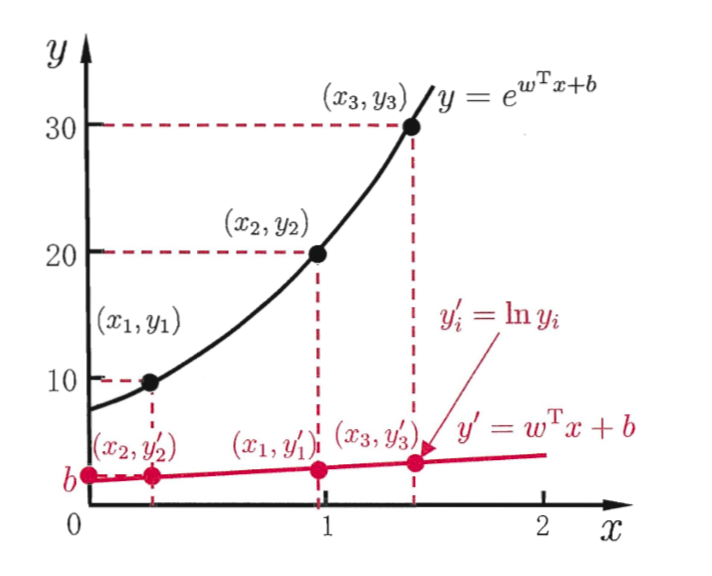
\includegraphics[width=0.5\textwidth]{\subfix{../images/log-linear-regression.png}}\par
  对数线性回归示意图
\end{figure}

通常而言,考虑单调可微函数 $g(\cdot)$,令
\begin{equation}
  y = g^{-1}(\pmb{w}^T\pmb{x} + b)
\end{equation}
这样得到的模型称为\textbf{广义线性模型(generalized linear model)},其中函数 $g(\cdot)$ 称为\textbf{联系函数(link function)}。
显然,对数线性回归是广义线性模型在 $g(\cdot) = \ln(\cdot)$ 时的特例。

注: 广义线性模型常用于回归任务。

\subsection{对数几率回归}

对于分类任务,只需要找一个单调可微函数将分类任务的真实标记 $y$ 与线性回归模型的预测值联系起来。

单位跃迁函数(unit-step function):
\begin{equation}
  y =
  \begin{cases}
    0,   & z < 0; \\
    0.5, & z = 0; \\
    1,   & z > 0;
  \end{cases}
\end{equation}

\begin{figure}[h]
  \centering
  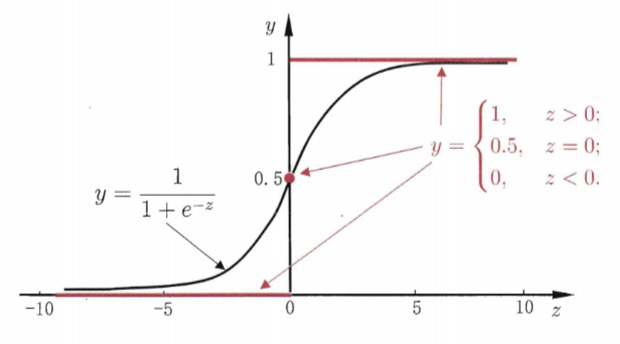
\includegraphics[width=0.6\textwidth]{\subfix{../images/unit-step-and-logistic.png}}\par
  单位跃迁函数与对数几率函数
\end{figure}

如图示,单位跃迁函数不连续,因此不能直接用作于式(3.15)中的 $g^-(\cdot)$。使用\textbf{对数几率函数(logistic function)}进行替代:
\begin{equation}
  y = \frac{1}{1+e^{-z}}
\end{equation}

对数几率函数是一种“Sigmoid 函数”,即\textit{将 $z$ 值转化为一个接近 $0$ 或 $1$ 的 $y$ 值,且其输出值在 $z=0$ 附近变化陡峭}。

将对数几率函数作为 $g^-(\cdot)$ 代入式(3.15),得:
\begin{equation}
  \begin{split}
    y & = g^{-1}(\pmb{w}^T\pmb{x}+b) \\
    & = \frac{1}{1 + e^{-\pmb{w}^T\pmb{x}+b}}
  \end{split}
\end{equation}

类似于式(3.14),式(3.18)可变化为
\begin{equation}
  \begin{split}
    y & = \frac{1}{1 + e^{-\pmb{w}^T\pmb{x}+b}} \\
    \frac{1}{y} & = 1 + e^{-\pmb{w}^T\pmb{x}+b} \\
    \frac{1-y}{y} & = e^{-\pmb{w}^T\pmb{x}+b} \\
    \frac{y}{1-y} & = e^{\pmb{w}^T\pmb{x}+b} \\
    \ln\frac{y}{1-y} & = \pmb{w}^T\pmb{x}+b
  \end{split}
\end{equation}

\textit{若将 $y$ 视为样本 $\pmb{x}$} 作为正例的可能性,那么 $1-y$ 则是其反例的可能性,两者的比值
\begin{equation}
  \frac{y}{1-y}
\end{equation}
称为\textbf{几率(odds)},反应了 $\pmb{x}$ 作为正例的相对可能性。对几率取对数则得到\textbf{对数几率(log odds,亦称 logit)}
\begin{equation}
  \ln\frac{y}{1-y}
\end{equation}

% TODO

\end{document}
